%# -*- coding: utf-8-unix -*-
%%==================================================
%% chapter03.tex for SJTU Bachelor Thesis
%%==================================================

%\bibliographystyle{sjtu2}%[此处用于每章都生产参考文献]
\chapter{测试与评估}
本章将分别对真实环境下的粗粒度调度器和仿真集群中的调度器设计与调优进行测试,并分析测试结果,从而得出结论。

\section{粗粒度调度算法的测试}
粗粒度调度算法基于Bash脚本实现(rebalance.sh),作为巨型虚拟机客户机的启动项运行在客户机中。巨型虚拟机部署在有四个节点的真实集群中,四个节点的配置如表\ref{tab:config}所示。每个节点有16个CPU核,128GB主存,节点之间通过网络相连。巨型虚拟机实例拥有32个vCPU,12G内存,每个节点上分别有8个本地vCPU。故巨型虚拟机给上层客户机呈现了一个NUMA架构的机器,共4个NUMA节点,分别为Node\,0-3,分别运行在Host\,0-3上。rebalance.sh脚本在客户机启动时首先将所有客户机内进程固定在Node\,0上,在此之后每隔2秒计算巨型虚拟机4个NUMA节点的steal time,如果当前处于活动状态的Node上steal time大于50个节拍,则将所有进程重新固定到steal time最低的节点。
\begin{table}[!htpb]
  \bicaption[测试集群配置]{测试集群配置}{Cluster Configuration in the Experiment}
  \label{tab:config}
  \centering
  \begin{threeparttable}[b]
     \begin{tabular}{c|c}
      \toprule
      \# of Machines & 4  \\
      \hline
      CPU & 16-core Intel Xeon CPU E5-2670 @ 2.60GHz  \\
      \hline
      DRAM & 128GB \\
      \hline
      Disk & SEAGATE ST9300605SS \\
      \hline
      Ethernet NIC & Broadcom NetXtreme BCM5720 Gigabit Ethernet \\
      \hline
      OS & Ubuntu 16.04 LTS \\
      \hline
      Kernel Version & Linux 4.9.76+ \\
      \bottomrule
    \end{tabular}
  \end{threeparttable}
\end{table}

为了测试巨型虚拟机的集群负载平衡能力,我们在Host\,0-3上分别启动了32个Memcached\cite{memcached}服务线程(Memcached Server),分别处理来自于Client\,0-3的Memcached写请求。Client端调用$libmemcached$库,每隔$gauss()$时间发出一批请求。在真实的工作负载中,客户端发送请求的间隔时间呈现高斯分布\footnote{高斯分布是常见的分布,详见https://en.wikipedia.org/wiki/Normal\_distribution},故我们的客户端也是经过每隔$gauss()$时间发送请求。如图\ref{fig:load},我们测量了Memcached服务器的工作负载在60秒内的变化情况,颜色越深表示工作负载越高。可以看出,Host\,3工作负载较其他三个Host更低,有大片的白色区域。这些白色区域是巨型虚拟机可以动态填补的区域,将白色区域分配给巨型虚拟机的工作负载将提高整个集群的CPU使用率。

\begin{figure}[!htp]
  \centering
  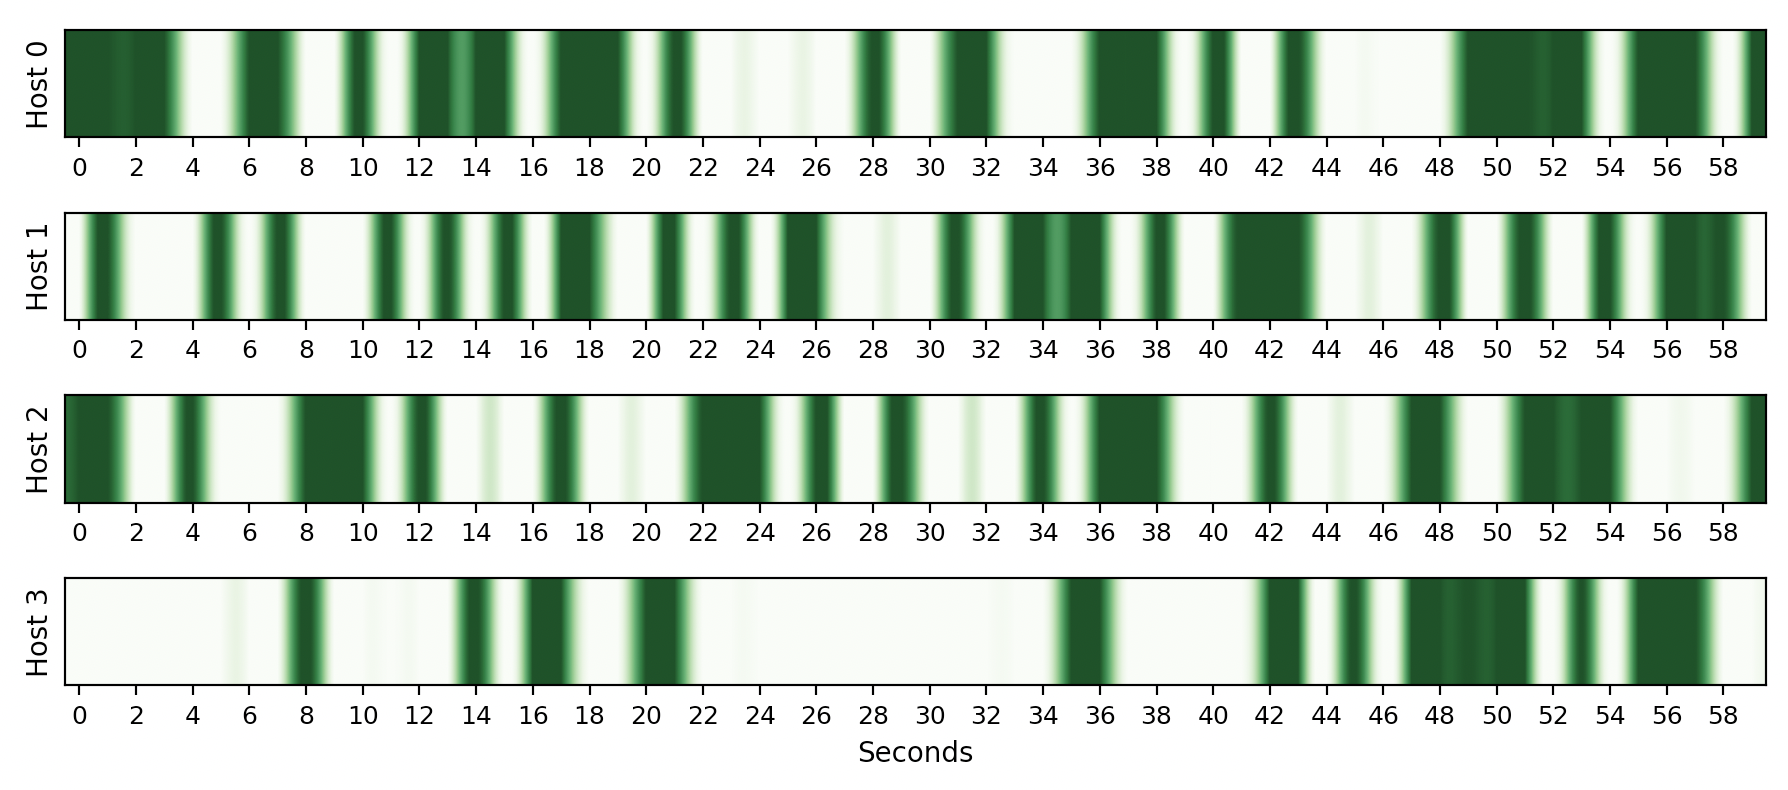
\includegraphics[width=14cm]{load.png}
  \bicaption[Memcached服务器负载波动]
    {Memcached服务器负载波动}
    {Fluctuation of Memcached Server Load}
  \label{fig:load}
\end{figure}

我们在巨型虚拟机中运行phoronix-test-suite\cite{phoronix}的pts/openssl benchmark作为尽力而为型任务,用于动态填补CPU使用率的空缺。Memcached属于延迟敏感型任务,我们测量Memcached的延迟来测量巨型虚拟机对延迟敏感型任务的影响程度。如图\ref{fig:latency},我们测量了每个Memcached写请求的Latency,并计算了整个过程中产生的所有Latency数据的平均数、95分位数、99分位数,用来全面的观察每个请求的延迟,以及尾延迟,还统计了整个测试过程中的请求处理速度QPS。与巨型虚拟机对比的对象是固定运行在Host\,0上的未修改的QEMU-KVM虚拟机(LC + Vanilla VM),具有8个vCPU,12G内存,以及没有虚拟机只有Memcached服务线程运行的情况(LC only)。可以看出,Vanilla VM对Memcached性能影响十分显著,而从延迟平均值看,巨型虚拟机对Memcached的影响微乎其微,只有在99分位数上有较大的影响。巨型虚拟机也未明显影响Memcached的QPS,每秒仅减少了10个左右的请求。

\begin{figure}[!htp]
  \centering
  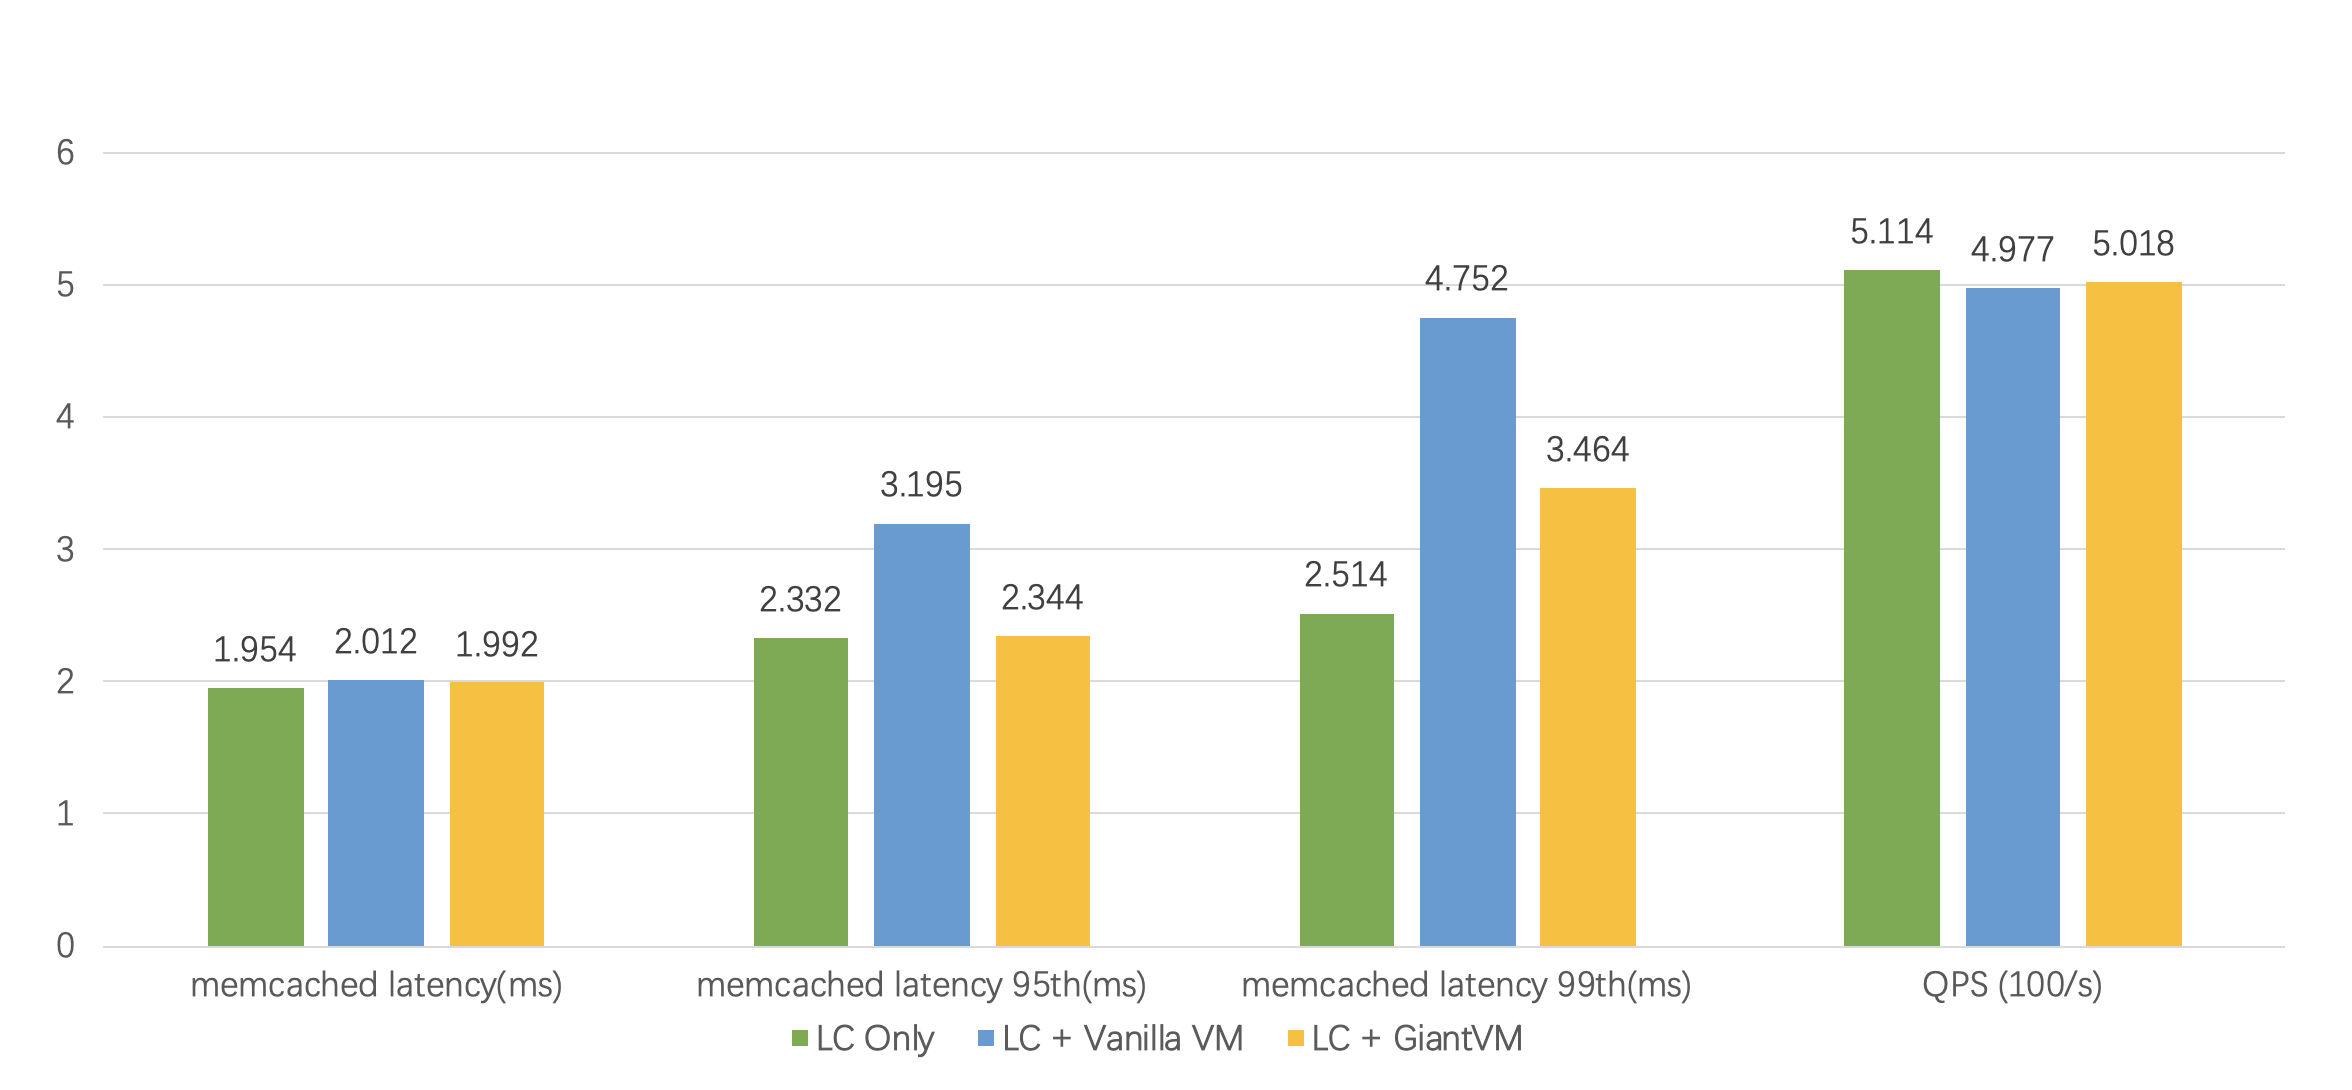
\includegraphics[width=15cm]{latency.png}
  \bicaption[Memcached请求性能比较]
    {Memcached请求性能比较}
    {Comparison of Memcached Requests Performance}
  \label{fig:latency}
\end{figure}
集群中CPU的负载均衡也是我们的设计目标。为此,我们记录了测试期间Host\,0-3上的CPU占用率变化情况,统计了平均值和基尼系数。如图\ref{fig:cpuload},相比于只运行Memcached服务线程的情况,Vanilla VM对集群总体的CPU利用率(即CPU的平均占用率)提升小于巨型虚拟机,CPU利用率的基尼系数相较于巨型虚拟机也更高。这是由于巨型虚拟机总是动态地迁移到CPU利用率低的节点,而普通虚拟机无法感知Host上的工作负载。pts/openssl测试结果也符合我们的设想,巨型虚拟机内每秒可完成714个签名(Signs),而普通虚拟机中只能完成708个,这说明,有迁移能力的虚拟机不但维持了宿主机上LC型任务的性能,还保持了客户机内BE型任务的性能。综上,真实环境下的巨型虚拟机调度器达到了设计目标。
\begin{figure}[!htp]
  \centering
  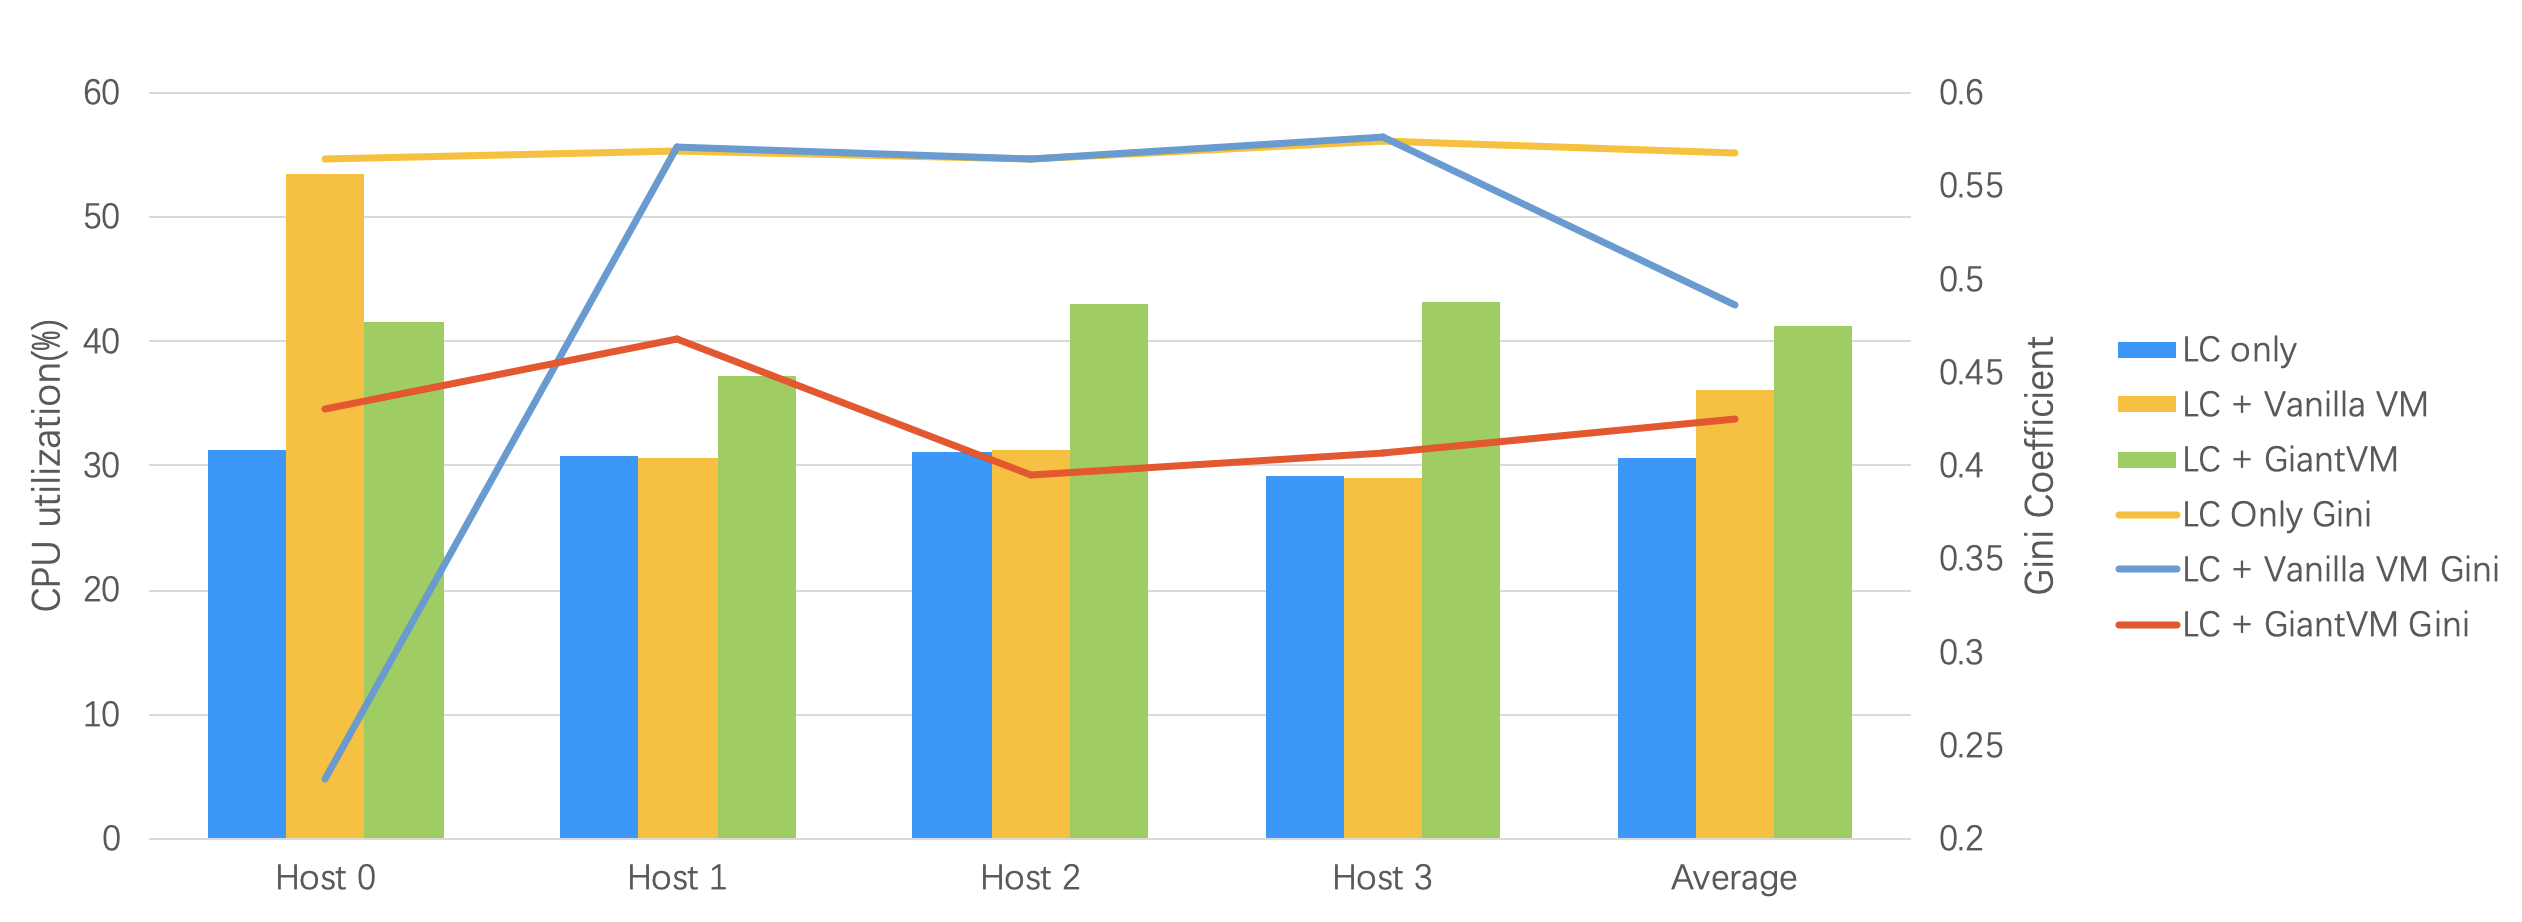
\includegraphics[width=16cm]{cpu.png}
  \bicaption[四个节点的CPU负载情况]
    {四个节点的CPU负载情况}
    {CPU Load of the Four Nodes}
  \label{fig:cpuload}
\end{figure}

\section{仿真环境下调度算法的对比测试}

本小节介绍仿真测试的测试环境并分析测试结果。仿真仅涉及集群进程数据的运算与处理,与具体的物理机配置无关,故只要有Python脚本的运行环境与谷歌的集群追踪数据即可运行仿真。

\begin{figure}[!htp]
  \centering
  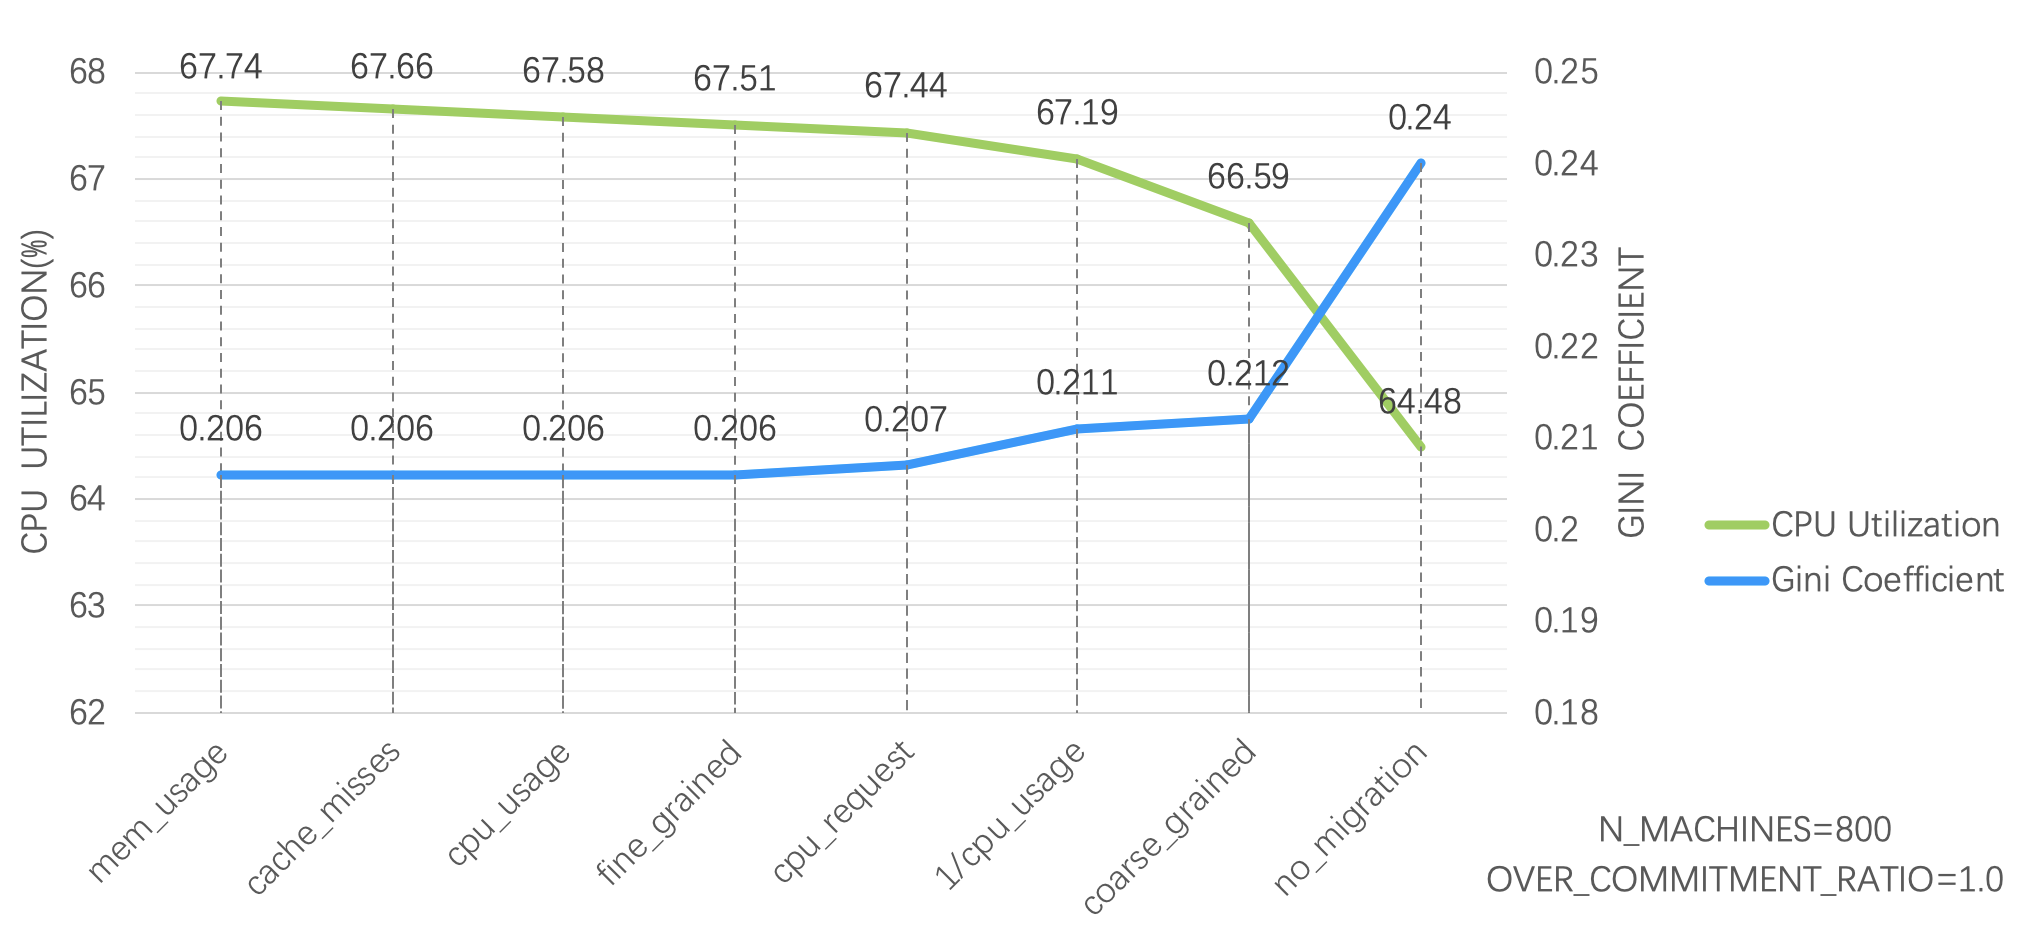
\includegraphics[width=14cm]{cpu_gini.png}
  \bicaption[调度算法CPU平衡效果对比]
    {调度算法CPU平衡效果对比}
    {Comparison of Scheduling Algorithms CPU Balancing Performance}
  \label{fig:cpu_gini}
\end{figure}
本文运行仿真脚本的Python版本是Python3.5.2,使用了Google clusterdata-2011-2其中的$task\_events$中part-00000-of-00500.csv到part-00009-of-00500.csv共10个csv数据表,以及$task\_usage$中的part-00000-of-00500.csv共1个csv数据表。我们没有使用更多的数据表,是因为数据加载时间过长,且这一部分数据量已经足够大,具有很好的代表性。

测试的可变参数有:(1)平衡策略,有:不平衡($no\_migration$)、粗粒度平衡($coarse\_grained$)、未排序的细粒度平衡($fine\_grained$)、根据CPU请求量排序的细粒度平衡($cpu\_request$)、根据CPU当前使用量排序的细粒度平衡($cpu\_usage$)、根据内存当前使用量排序的细粒度平衡($mem\_usage$)、根据CPU当前使用量逆排序(从大到小)的细粒度平衡($1/cpu\_usage$)、根据当前缓存不命中频率排序的细粒度平衡($cache\_misses$)(2)集群机器数量:任务数量不可变,通过更改集群机器数量配置测试调度脚本性能;(3)资源超量供应系数($overcommitment\,ratio$):指调度器真实分配给进程的资源与进程资源请求量的比例。此比例越高,则表明调度器给每个进程提供的超额资源越多,系统资源竞争越小,反之资源竞争越激烈。

如图\ref{fig:cpu_gini}所示,我们首先固定机器个数为800,$overcommitment\,ratio$为1.0,对比所有调度算法的性能。此时任务的数量不变,集群机器数量也不变。可见,不平衡的调度算法性能最差,其次是粗粒度的调度算法。在细粒度的调度算法中,未排序的算法性能没有明显下降,这是由于测试的随机性;而优先调度$CPU\,usage$较高的算法在细粒度算法中效果最差,符合我们的预期;而按照内存指标排序的算法的性能普遍高于按照CPU指标排序,这是因为在集群中迁移内存占用较大的进程会造成更大的性能损失与网络开销。而基尼系数的变化趋势则与CPU的变化趋势相反,这是由于集群机器数量和任务数量不变,越平衡的调度算法CPU使用率越高,基尼系数越小。

\begin{figure}[!htp]
  \centering
  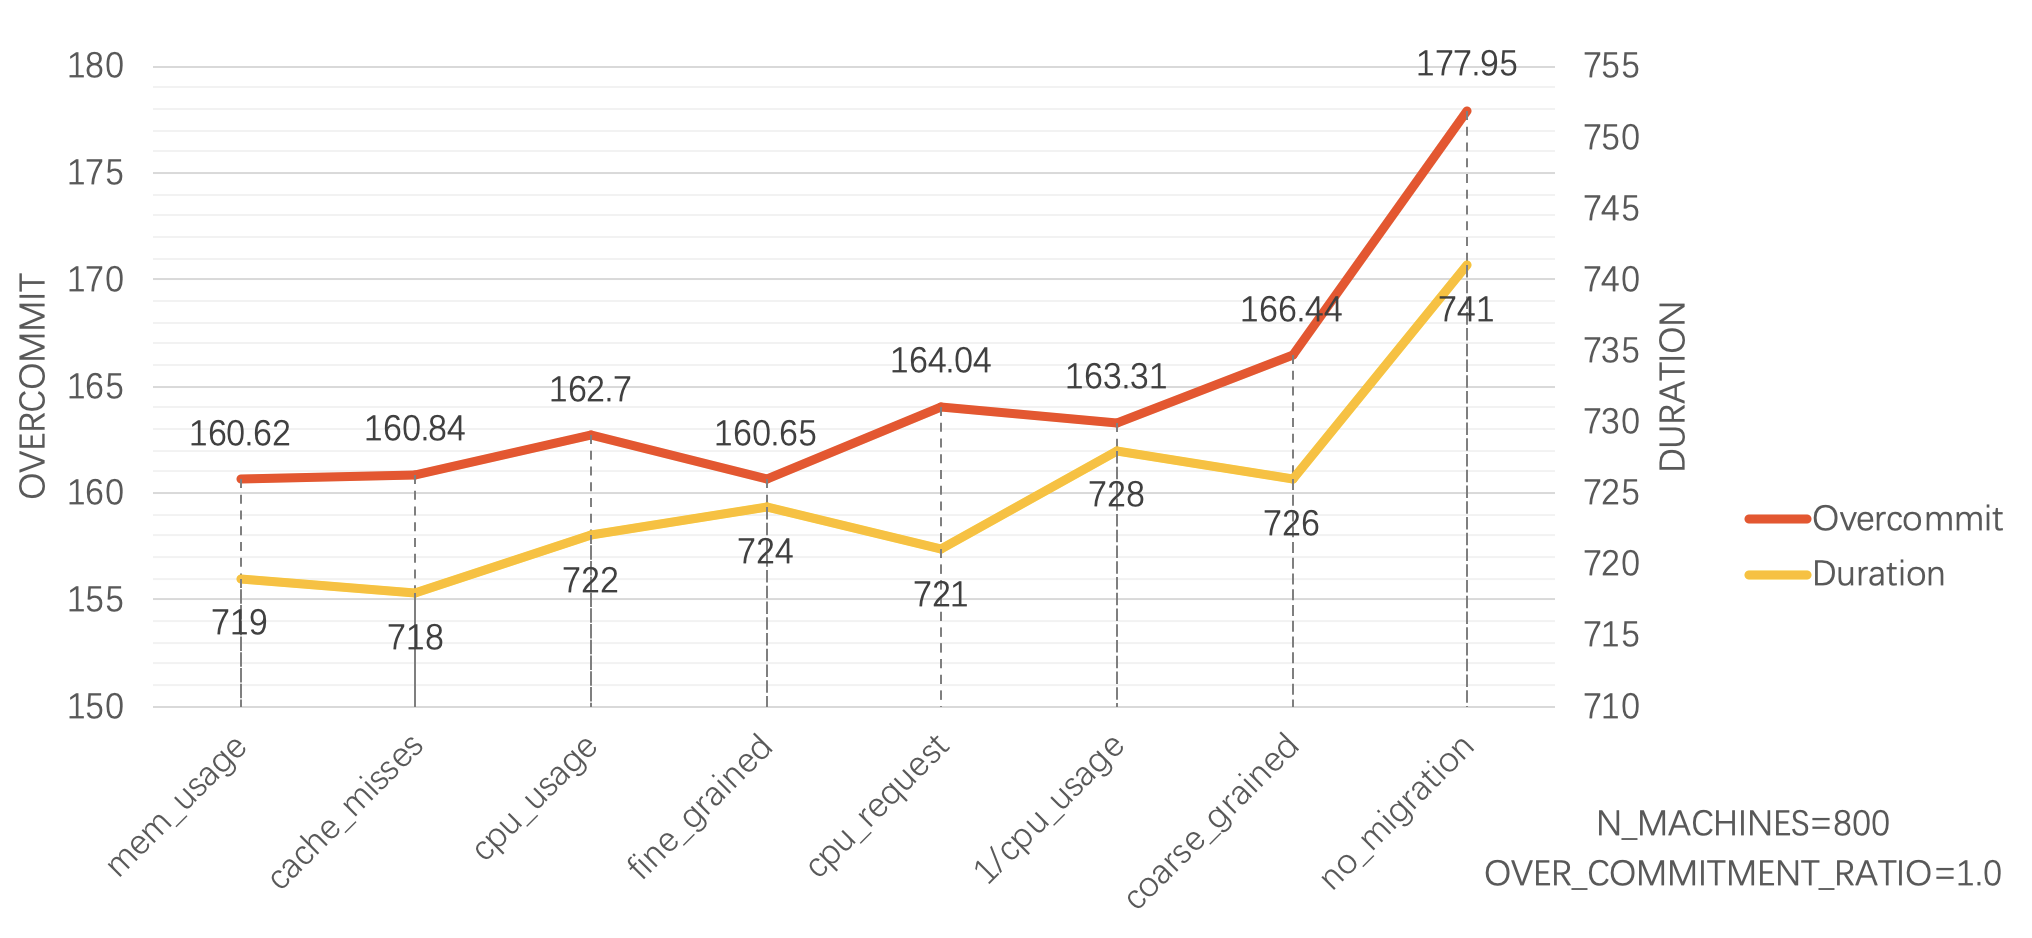
\includegraphics[width=14cm]{dur_over.png}
  \bicaption[调度算法任务性能对比]
    {调度算法任务性能对比}
    {Comparison of Task Performance in Scheduling Algorithms}
  \label{fig:dur_over}
\end{figure}

本文除了CPU和基尼系数两个测试指标之外,还有两个测试指标:所有任务的平均超量使用资源(Overcommit),以及所有任务的平均延迟(Duration)。这三项指标均是越低越好,网络带宽占用小的调度算法对集群其他工作负载影响小;任务的超量使用资源越少,则表明在真实的集群中该任务的QoS影响越小,调度算法平衡性能更强;任务的延迟越小,则表明任务等待调度的时间越短,即获得了更多的运行时间。如图\ref{fig:dur_over}所示,横轴调度算法的顺序与图\ref{fig:cpu_gini}相同,两项指标虽然有起伏,但总体在升高,和我们测得的CPU与基尼系数两项数据大致吻合。

调度算法的网络开销也是我们关注的重点。对于网络带宽占用,我们统计了每个迁移循环的网络开销,并将数据做累积,计算从开始集群仿真到每个迁移循环为止的网络用量。如图\ref{fig:minetwork},仿真集群开始运行时,网络开销较小,这是由于集群的任务数量尚未填满,无需进行调度。其后进程数量逐渐增多,调度的网络开销也增加,直到最后进程逐渐完成,集群负载再次下降,调度的网络开销也逐渐变小。对不同的调度算法进行对比,粗粒度的调度算法网络开销最大,由于每个循环中迁移的进程数目较多;不做迁移则网络开销为0,按照缓存不命中排序的算法网络开销最小,由于MPI真实地反映了进程频繁访问页面的多少。按照CPU指标排序的算法的网络开销普遍大于按照Memory指标排序的算法,这也是我们预期之内的。
\begin{figure}[!htp]
  \centering
  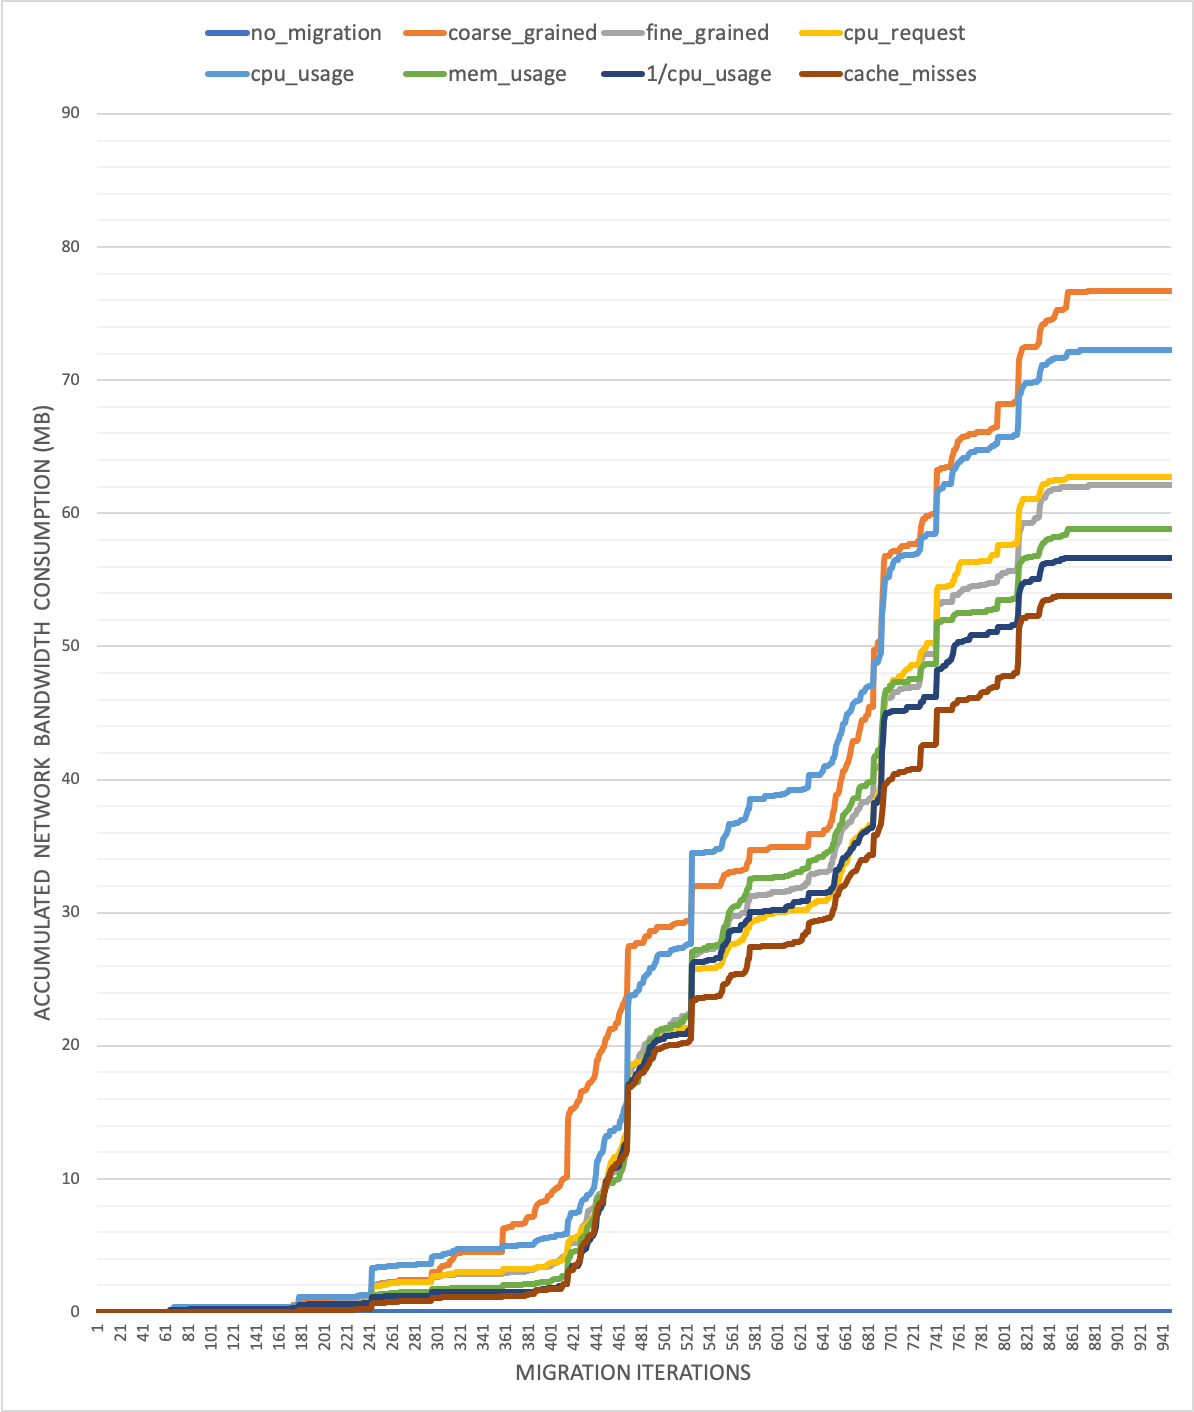
\includegraphics[width=10cm]{network.png}
  \bicaption[调度算法网络开销对比]
    {调度算法网络开销对比}
    {Comparison of Scheduling Algorithms' Network Overhead}
  \label{fig:minetwork}
\end{figure}

\begin{figure}[!htp]
  \centering
  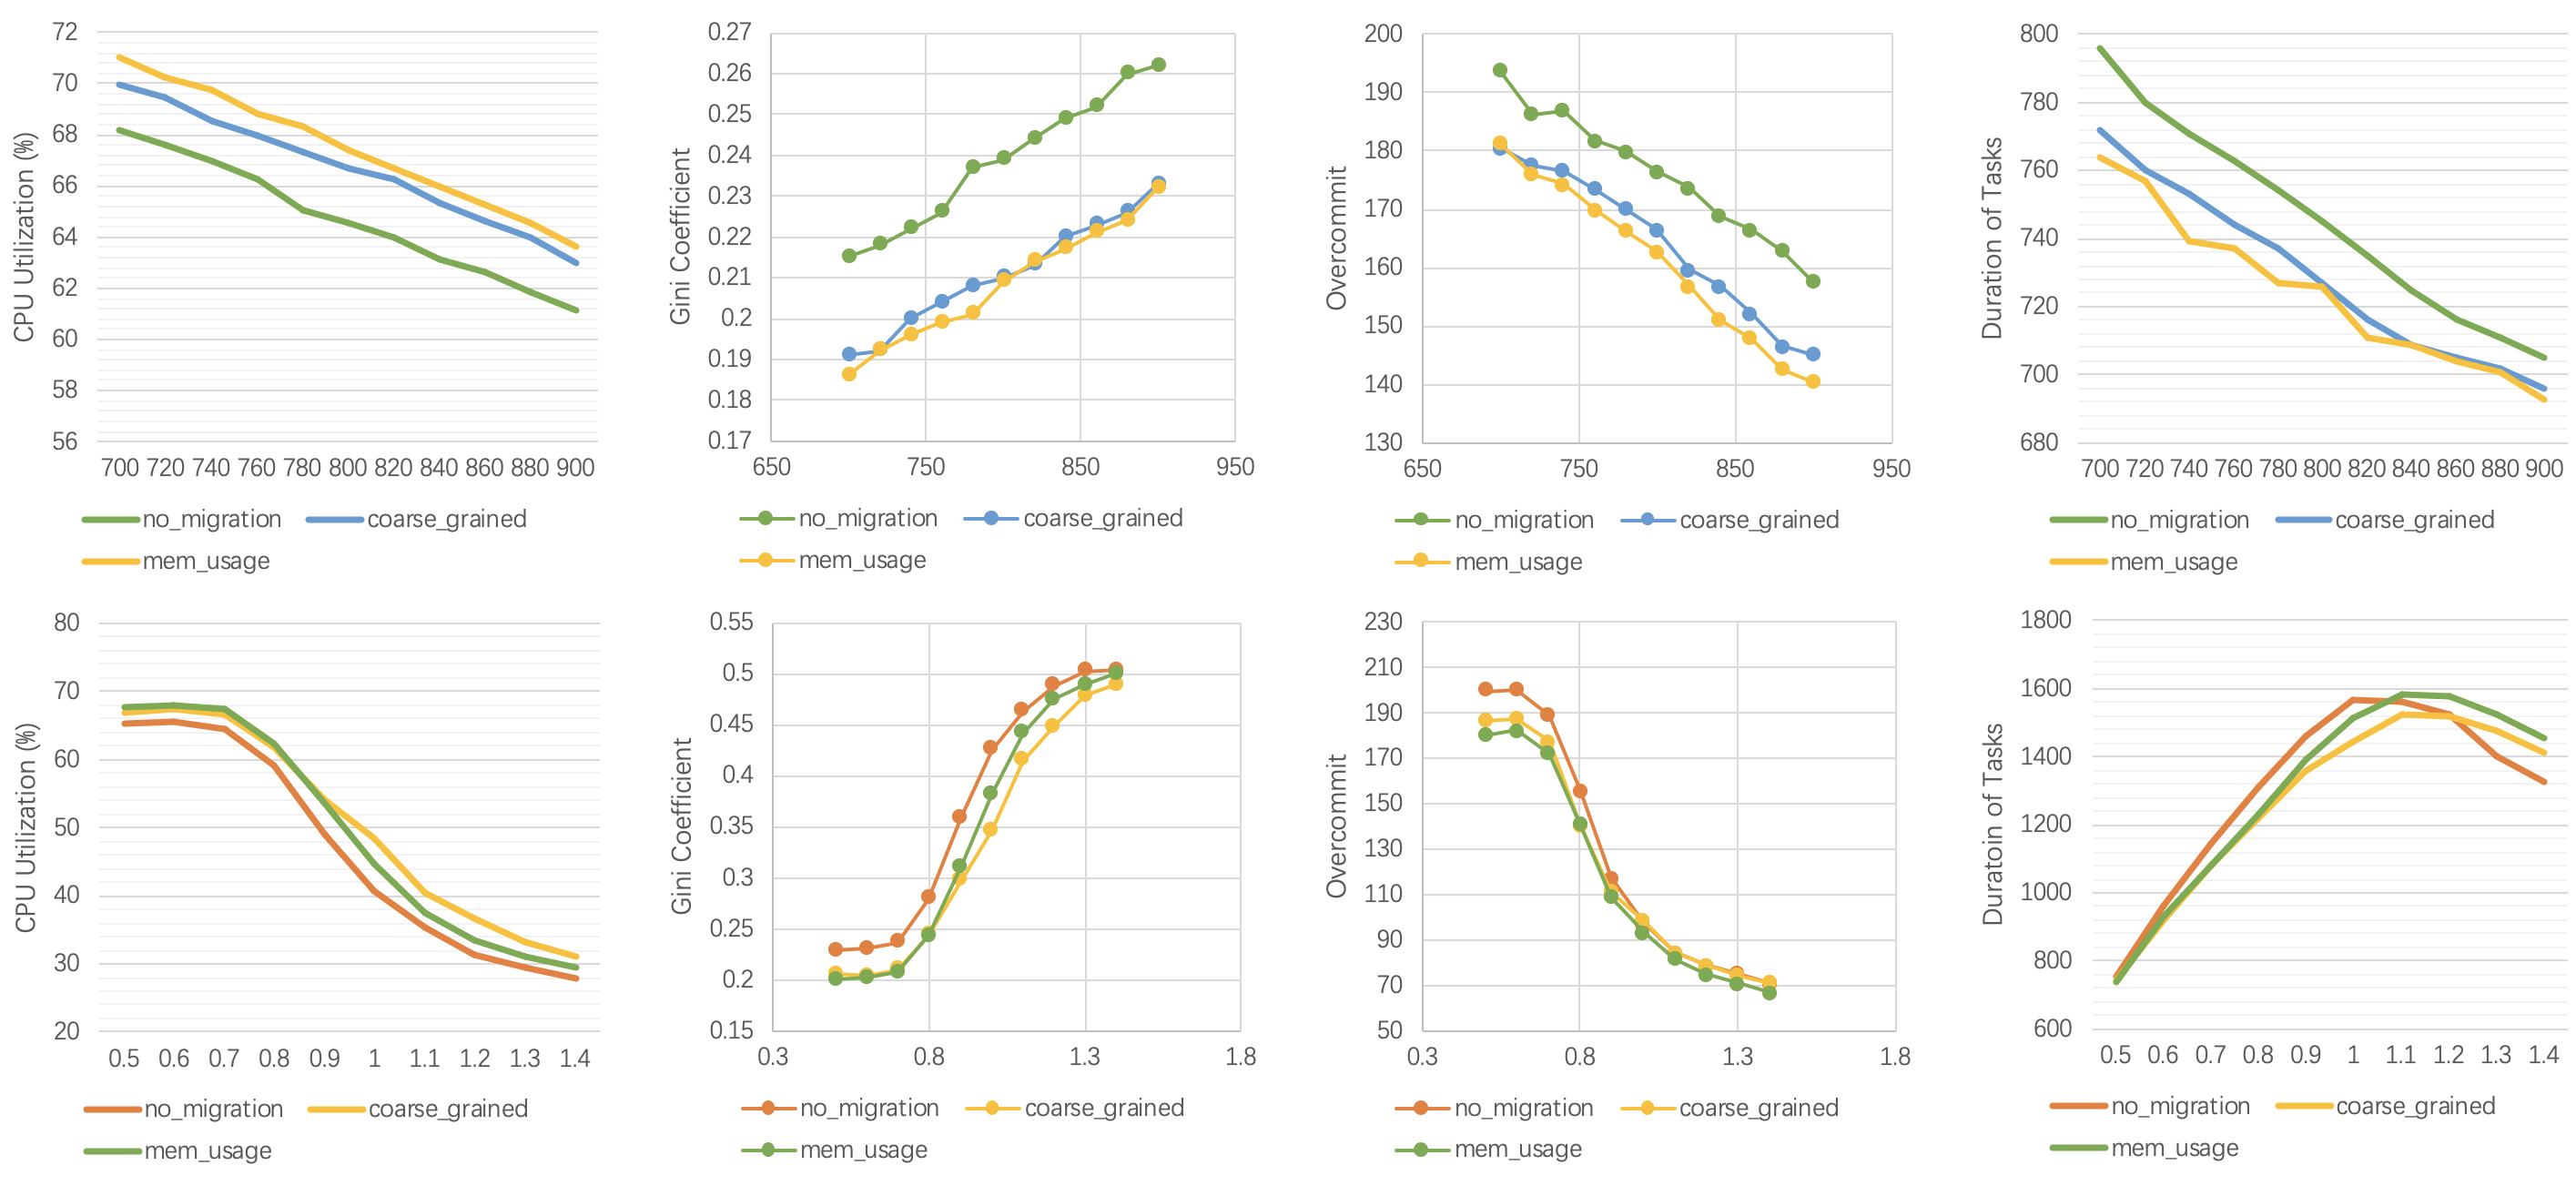
\includegraphics[width=16cm]{compare.png}
  \bicaption[变更参数对调度算法的影响]
    {变更参数对调度算法的影响}
    {Influences of Parameter Changing to Scheduling Algorithms}
  \label{fig:comparing}
\end{figure}

我们还测试了不同的集群大小($N\_MACHINES$)和资源超量提供率($Over\_commitment\_ratio$)对调度算法各项指标的影响。如图\ref{fig:comparing},第一行改变集群机器的数量(从700到900),第二行改变资源超量提供率(从0.5到1.4),来测试对CPU使用率、基尼系数、资源超量使用量、延迟的影响。可以看出,无论是改变机器数量还是改变资源超量提供率,不使用平衡算法的随机调度各项指标均是最差的,而粗粒度的调度算法和细粒度算法(我们使用对内存用量进行排序的细粒度算法做对比)性能较为接近。在变化机器数量的测试中,细粒度的算法要优于粗粒度的算法。而变化资源超量提供率的测试中,粗粒度算法要优于细粒度算法,这个现象的原因尚未查明。

\begin{figure}[!htp]
  \centering
  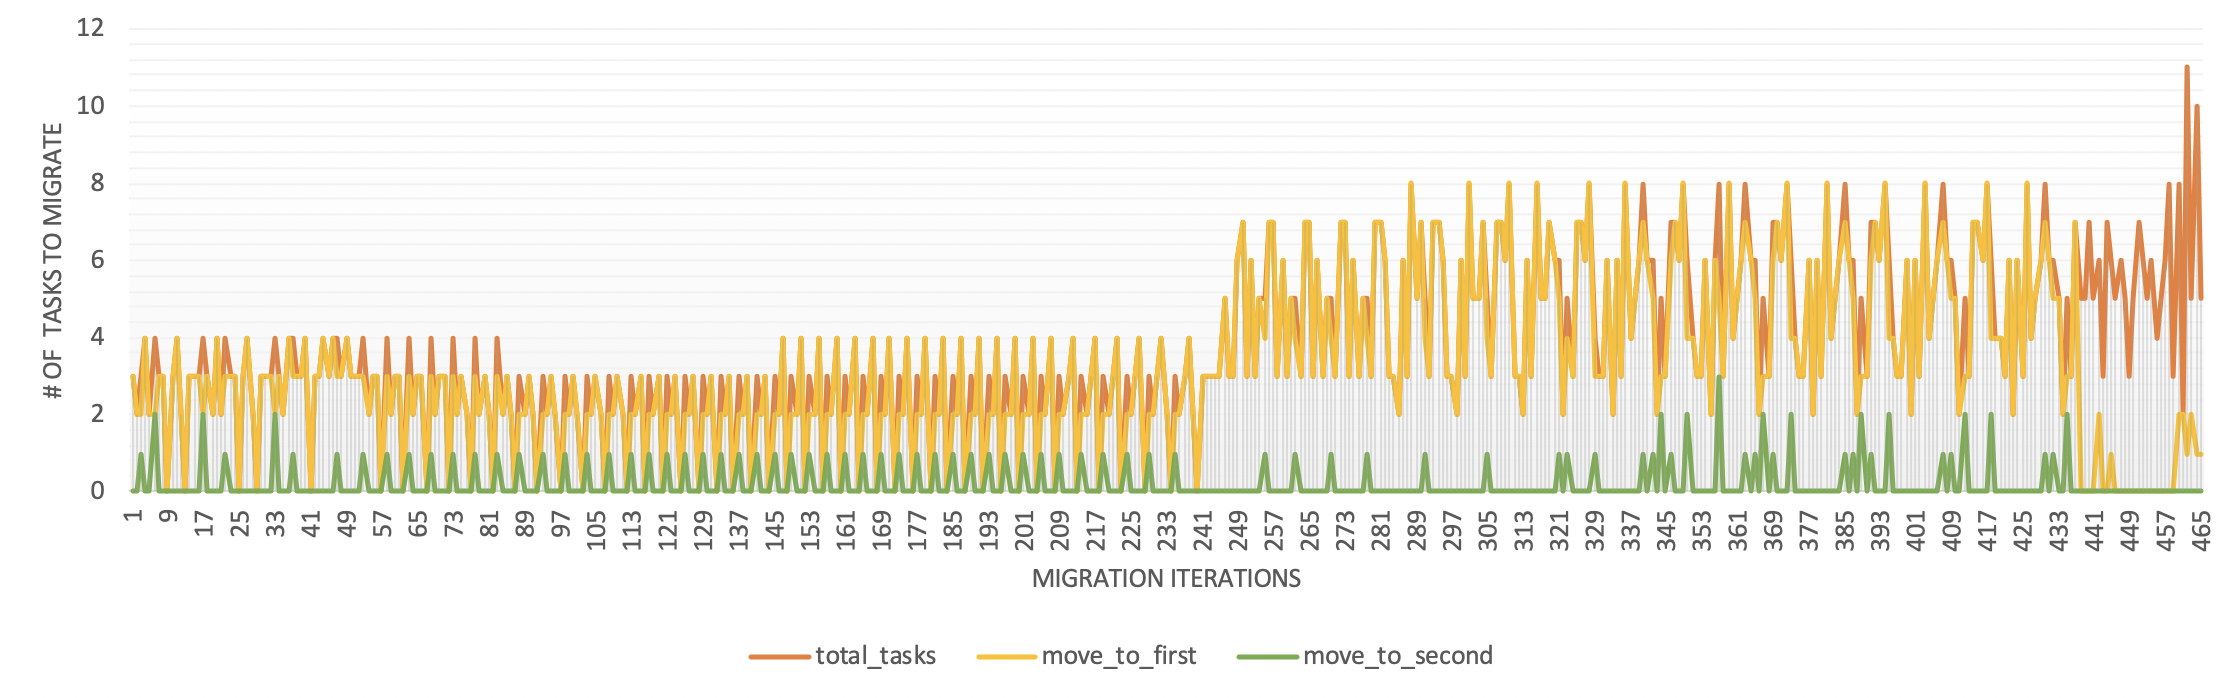
\includegraphics[width=16cm]{tasks.png}
  \bicaption[细粒度调度算法迁移进程分布]
    {细粒度调度算法迁移进程分布}
    {Distribution of Migrated Task in Fine-Grained Scheduling Algorithm}
  \label{fig:distr}
\end{figure}

最后,我们测试细粒度算法是否需要进行更细粒度的优化。我们选取根据$mem\_usage$排序的细粒度调度算法进行测试,由于其CPU负载平衡性能最佳。如图\ref{fig:distr},$total\_tasks$表示一个$G\_cell$中所有待迁移的进程,而$move\_to\_first$代表被调度到负载最低的节点上的进程数量,$move\_to\_second$代表被调度到负载第二低的节点上的进程数量,故在每个迁移循环中,有$total\_tasks\,=\,move\_to\_first\,+\,move\_to\_second$。可以看出,对于大小为4的$G\_cell$,$move\_to\_first$已经占据了绝大部分的可迁移进程,而$move\_to\_second$使用了剩余的可迁移进程,故CPU平衡性能较粗粒度的调度算法更好,但不需要考虑负载第三低节点,由于给负载第二低的节点剩余的进程已经很少,可以推知负载第三低节点已经没有可使用的进程。而对于其他大小的$G\_cell$,存在一个最佳的调度粒度,本文尚未进行研究。

\section{本章小结}
本章首先对真实环境下的粗粒度调度脚本进行了测试,分别在巨型虚拟机和物理节点上运行尽力而为型和延迟敏感型任务,得知粗粒度的调度算法可以动态感知工作负载的变化,提高集群CPU使用率,对任务服务质量的影响较低,以一种高效的方式完成了资源重分配,达到了我们的设计目标。同时,我们对仿真集群中的各类调度算法进行了测试,得知细粒度的调度算法比粗粒度的算法更优,而对进程排序更有效地优化了细粒度调度算法的性能。我们还探讨了是否需要更细粒度的优化,经过对可迁移进程的分布进行统计,我们发现无需进行更细粒度的优化。
